% =============================================================
%  VVSC_Chuang_ChengShun_HW4.tex
%  AOE/CS/ME 6444 — Verification and Validation in Scientific Computing
%  Homework #4 — Solution Verification
%  Spring 2026 | Dr. Chris Roy
%  Authors: Jason Cusati & Cheng-Shun Chuang
% =============================================================
\documentclass[11pt,letterpaper]{article}

\usepackage[margin=1in,headheight=14pt]{geometry}
\usepackage{amsmath,amssymb}
\usepackage{booktabs}
\usepackage{graphicx}
\usepackage{xcolor}
\usepackage{hyperref}
\usepackage{caption}
\usepackage{subcaption}
\usepackage{array}
\usepackage{multirow}
\usepackage{parskip}
\usepackage{float}
\usepackage{enumitem}
\usepackage{fancyhdr}

\hypersetup{colorlinks=true, linkcolor=blue, citecolor=blue, urlcolor=blue}

% ── header / footer ────────────────────────────────────────────────────────
\pagestyle{fancy}
\fancyhf{}
\rhead{AOE/CS/ME 6444 — HW\,4}
\lhead{Cusati \& Chuang}
\cfoot{\thepage}

% ── custom column type ─────────────────────────────────────────────────────
\newcolumntype{R}[1]{>{\raggedleft\arraybackslash}p{#1}}

% ── macros ─────────────────────────────────────────────────────────────────
\newcommand{\UDE}{U_{\mathrm{DE}}}
\newcommand{\UIT}{U_{\mathrm{IT}}}
\newcommand{\URO}{U_{\mathrm{RO}}}
\newcommand{\UNUM}{U_{\mathrm{NUM}}}
\newcommand{\pobs}{\hat{p}}
\newcommand{\pth}{p_{\mathrm{th}}}
\newcommand{\EI}{EI}
\newcommand{\GCI}{\mathrm{GCI}}
\newcommand{\fRE}{f_{\mathrm{RE}}}

% =============================================================
\begin{document}

% ── Title ──────────────────────────────────────────────────────────────────
\begin{center}
  {\LARGE\bfseries Homework \#4: Solution Verification}\\[6pt]
  {\large AOE/CS/ME 6444 — Verification and Validation in Scientific Computing}\\
  {\large Spring 2026 \quad|\quad Instructor: Dr.\ Chris Roy}\\[4pt]
  {\large Jason Cusati \quad\&\quad Cheng-Shun Chuang}\\[2pt]
  {\normalsize Due: Thursday, April 9, 2026}
\end{center}
\vspace{6pt}
\hrule
\vspace{10pt}

% =============================================================
\section{Introduction and Application Description}
\label{sec:intro}

This report presents a solution verification study for an \textbf{Euler–Bernoulli (EB)
finite-difference beam solver} applied to the structural assessment of a residential
wood header.  The same physical case will serve as the basis for the subsequent
uncertainty quantification (UQ) studies in Homework~5.

\subsection*{Physical Case}

An 8-ft simply-supported LVL (laminated veneer lumber) header carries a uniform
distributed load representative of residential roof framing:

\begin{center}
\begin{tabular}{llll}
  \toprule
  Parameter & Symbol & Value & Units \\
  \midrule
  Span            & $L$      & 96.0   & in \\
  Width           & $b$      & 3.5    & in \\
  Depth           & $d$      & 11.25  & in \\
  Elastic modulus & $E$      & 2,000,000 & psi \;(Microllam 2.0E, ESR-1387) \\
  Uniform load    & $q_0$    & 500    & lb/ft \;(= 41.667 lb/in) \\
  Flexural rigidity & $\EI$ & $8.3057\times10^8$ & lb$\cdot$in$^2$ \\
  \bottomrule
\end{tabular}
\end{center}

\subsection*{Governing Equation and Boundary Conditions}

The beam is governed by the 4th-order EB BVP with simply-supported ends:
\begin{equation}
  \EI\,w''''(x) = q_0,\quad x\in(0,L);
  \qquad
  w(0)=w(L)=0,\quad w''(0)=w''(L)=0.
  \label{eq:bvp}
\end{equation}

\subsection*{Numerical Method}

Equation~\eqref{eq:bvp} is discretized using a 5-point central-difference stencil
on a uniform grid of $N$ intervals ($N+1$ nodes):
\begin{equation}
  \frac{\EI}{h^4}\bigl(w_{i-2}-4w_{i-1}+6w_i-4w_{i+1}+w_{i+2}\bigr) = q_0,
  \quad i=2,\ldots,N-2,
  \label{eq:stencil}
\end{equation}
with modified near-boundary rows for the simply-supported ghost-node conditions.

\subsubsection*{Formal Order of Accuracy ($\pth=2$)}

Expanding each shifted value about node $x_i$ via Taylor series (terms
through $\mathcal{O}(h^8)$ shown):
\begin{equation}
  w_{i\pm k} = w_i \pm kh\,w_i' + \tfrac{(kh)^2}{2!}w_i''
               \pm \tfrac{(kh)^3}{3!}w_i'''
               + \tfrac{(kh)^4}{4!}w_i''''
               \pm \tfrac{(kh)^5}{5!}w_i^{(5)}
               + \tfrac{(kh)^6}{6!}w_i^{(6)} + \cdots
\end{equation}
Substituting $k=1,2$ with their signed coefficients $(-4, +1)$ into the
stencil numerator and collecting by derivative order, all odd-derivative
and even-derivative terms below order~4 cancel identically:
\begin{align}
  w_{i-2}-4w_{i-1}+6w_i-4w_{i+1}+w_{i+2}
  &= h^4\,w_i'''' + \frac{h^6}{6}\,w_i^{(6)} + \mathcal{O}(h^8).
  \label{eq:taylor}
\end{align}
Dividing~\eqref{eq:taylor} by $h^4$ and multiplying by $\EI$ gives the
\emph{local truncation error} (LTE):
\begin{equation}
  \tau_i = \EI\,w_i'''' + \underbrace{\frac{\EI\,h^2}{6}\,w_i^{(6)}
            + \mathcal{O}(h^4)}_{\text{LTE}} - q_0
         = \frac{\EI\,h^2}{6}\,w_i^{(6)} + \mathcal{O}(h^4),
\end{equation}
since $\EI\,w'''' = q_0$ by the governing equation.
Therefore the scheme is formally second-order accurate, $\pth = 2$, and the
global discretization error satisfies $|e_h| \sim C\,h^2$ as $h\to 0$.
The resulting linear system $Kw=q$ is solved directly with dense LU factorisation
(\texttt{numpy.linalg.solve}).  \textbf{There is no iterative solver;
iterative error is therefore identically zero.}

\subsection*{System Response Quantities (SRQs)}

Three SRQs are tracked:
\begin{enumerate}[nosep]
  \item $w_{\max}$ — peak mid-span deflection [in]
  \item $M_{\max}$ — peak bending moment [lb$\cdot$in], computed from $M=-\EI w''$
  \item $\sigma_{\max}$ — peak bending stress [psi]$= M_{\max}/S$, where $S$ is the section modulus
\end{enumerate}

\subsection*{Closed-Form References}

The exact solution for uniform load on a simply-supported beam is:
\begin{equation}
  w_{\mathrm{exact}}(x)=\frac{q_0}{24\EI}\bigl(x^4-2Lx^3+L^3 x\bigr),
\end{equation}
yielding the reference SRQ values used only to interpret results (not used
in the GCI analysis):
\[
  w_{\max}^{\mathrm{exact}}=0.05548021\ \text{in},\quad
  M_{\max}^{\mathrm{exact}}=48000.00\ \text{lb}\cdot\text{in},\quad
  \sigma_{\max}^{\mathrm{exact}}=650.1587\ \text{psi}.
\]

% =============================================================
\section{Grid Convergence Study}
\label{sec:grids}

Five systematically-refined grids are employed with constant refinement ratio
$r=h_{\mathrm{coarse}}/h_{\mathrm{fine}}=2$:

\begin{center}
\begin{tabular}{ccccccc}
  \toprule
  Level & $N$ & $h$ [in] & $w_{\max}$ [in] & $M_{\max}$ [lb$\cdot$in] & $\sigma_{\max}$ [psi] \\
  \midrule
  1 (coarsest) & 10  & 9.600 & 0.0559241 & 48000 & 650.159 \\
  2            & 20  & 4.800 & 0.0555912 & 48000 & 650.159 \\
  3            & 40  & 2.400 & 0.0555079 & 48000 & 650.159 \\
  4            & 80  & 1.200 & 0.0554871 & 48000 & 650.159 \\
  5 (finest)   & 160 & 0.600 & 0.0554819 & 48000 & 650.159 \\
  \midrule
  Exact        & $\infty$ & 0 & 0.0554802 & 48000.00 & 650.1587 \\
  \bottomrule
\end{tabular}
\end{center}

The requirement of \emph{at least four} systematically refined grids is satisfied
by five levels (four refinement steps at $r=2$ each).
Figure~\ref{fig:gci} shows the SRQ convergence with GCI uncertainty bands.
Figures~\ref{fig:de_error}--\ref{fig:roundoff_error} provide dedicated plots for each
uncertainty source ($\UDE$, $\UIT$, $\URO$) separately.

\begin{figure}[ht]
  \centering
  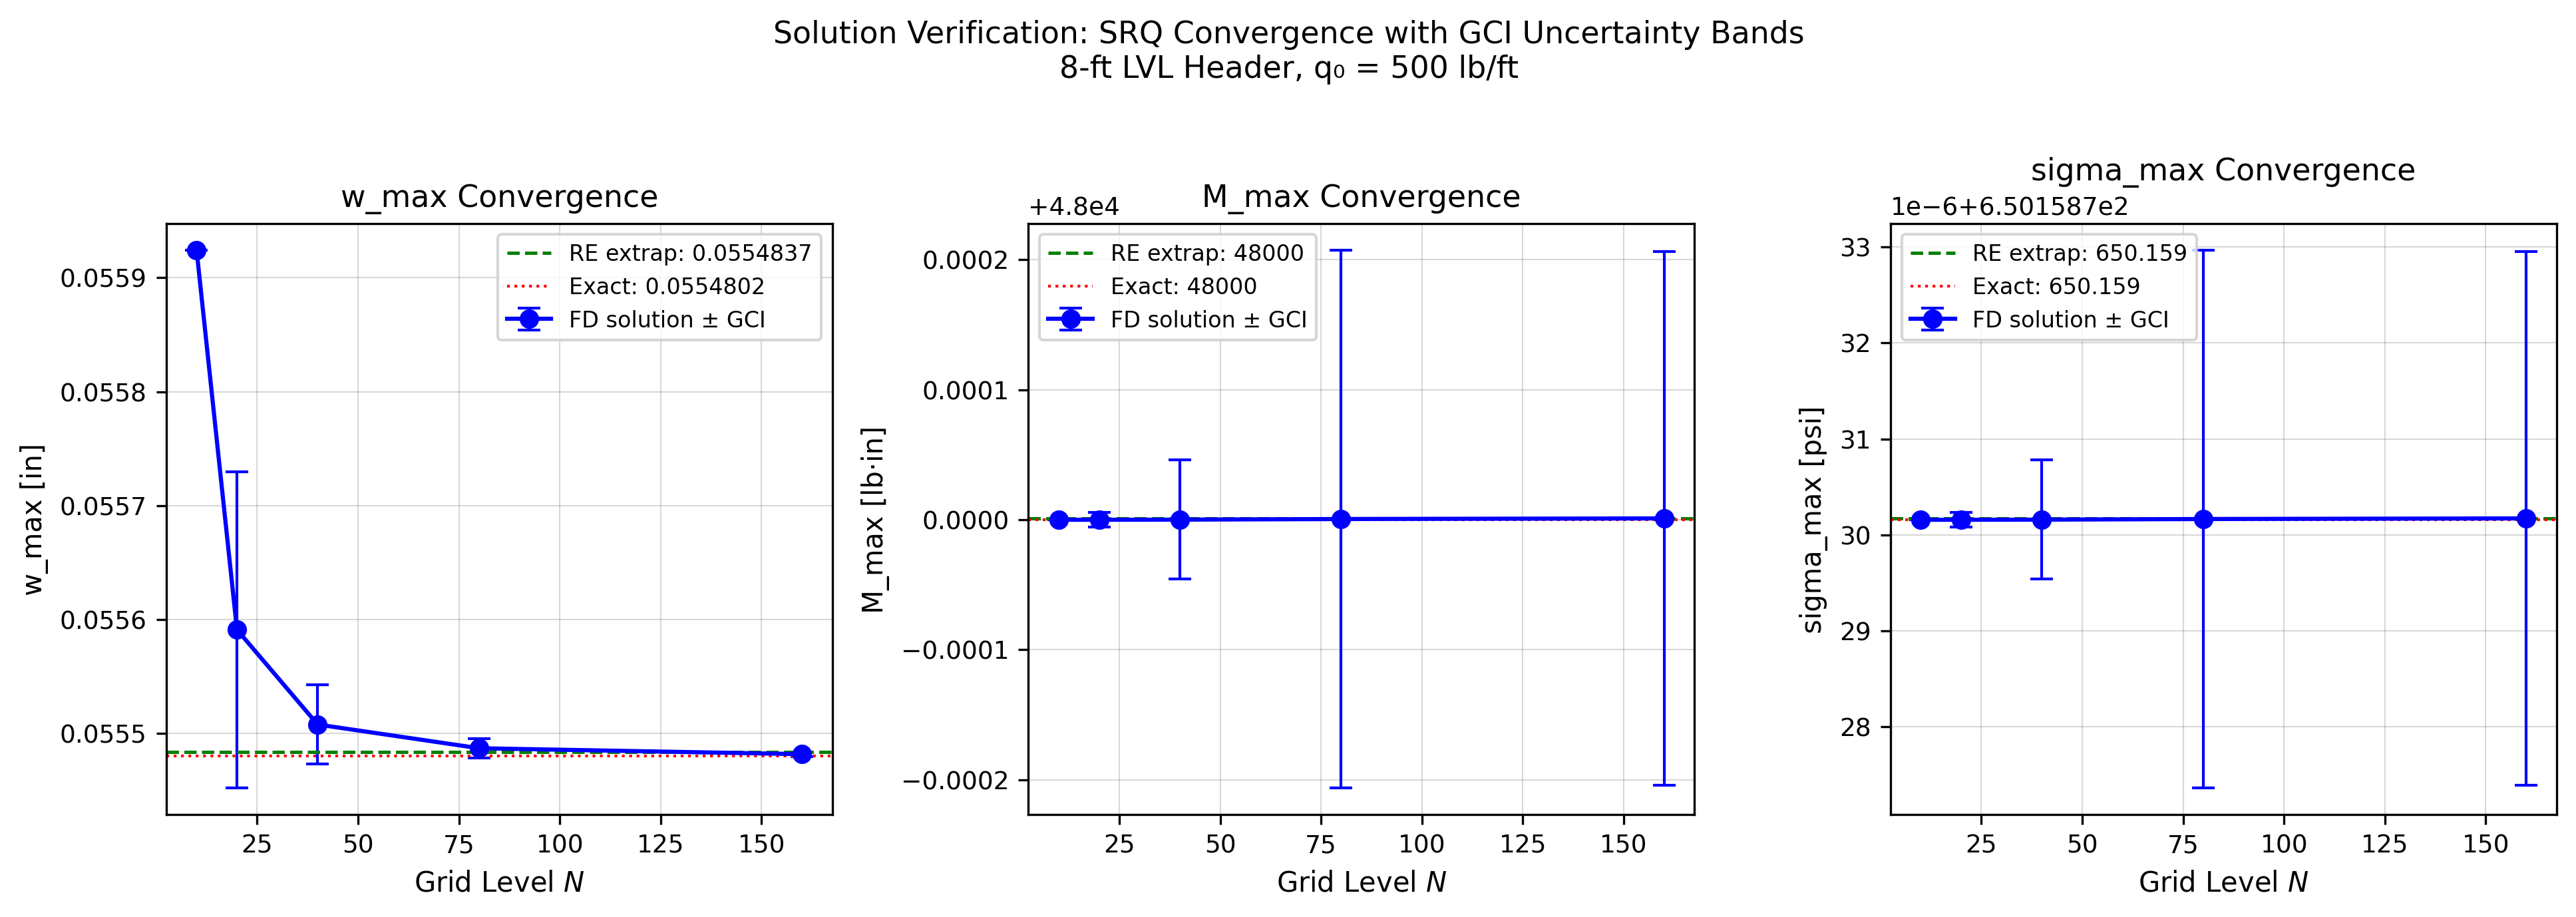
\includegraphics[width=\textwidth]{figures/fig1_convergence_gci.png}
  \caption{SRQ values versus grid level $N$ with GCI uncertainty bands ($\pm\UDE$)
    and Richardson-extrapolated estimates (\textcolor{green}{green dashes}).
    The \textcolor{red}{red dotted} line marks the exact solution.
    Left: $w_{\max}$; centre: $M_{\max}$; right: $\sigma_{\max}$.}
  \label{fig:gci}
\end{figure}

% =============================================================
\section{Discretization Error: Richardson Extrapolation and GCI}
\label{sec:gci}

\subsection{Methodology}

For every consecutive triplet of grids $(f_1, f_2, f_3)$ with $h_2=rh_1$,
$h_3=r^2 h_1$, the observed order of accuracy is:
\begin{equation}
  \pobs = \frac{\ln\!\left(|f_3-f_2|\,/\,|f_2-f_1|\right)}{\ln r}.
  \label{eq:pobs}
\end{equation}
The Richardson-extrapolated value is:
\begin{equation}
  \fRE = f_1 + \frac{f_2-f_1}{r^{\pobs}-1}.
  \label{eq:re}
\end{equation}
The Grid Convergence Index (GCI) provides the uncertainty in $f_1$ due to
discretization:
\begin{equation}
  \UDE = \GCI_{12} = F_s\,\frac{|f_2-f_1|}{r^{\pobs}-1},
  \label{eq:gci}
\end{equation}
where the factor of safety $F_s$ is set per Roy's criterion:
\begin{equation}
  F_s =
  \begin{cases}
    1.25 & \text{if } 0.5 \le \pobs/\pth \le 2.0 \quad\text{(asymptotic, reliable)},\\
    3.00 & \text{otherwise} \quad\text{(not in asymptotic regime)}.
  \end{cases}
  \quad \pth = 2.
  \label{eq:fs}
\end{equation}
Asymptotic convergence is confirmed when:
\begin{equation}
  \mathrm{ratio} = \frac{\GCI_{23}}{r^{\pobs}\,\GCI_{12}} \approx 1.
  \label{eq:asym}
\end{equation}

\subsection{Results — \texorpdfstring{$w_{\max}$}{w\_max}}

$w_{\max}$ exhibits clean monotone convergence.  All triplet analyses yield
$\pobs\approx 2.000 = \pth$, confirming the $\mathcal{O}(h^2)$ scheme is
operating in its asymptotic regime.  Consequently $F_s=1.25$ applies throughout.

\begin{table}[h!]
\centering
\caption{GCI analysis for $w_{\max}$ [in]. Exact $= 0.0554802$~in.}
\label{tab:gci_w}
\small
\begin{tabular}{lrrrrrrrrr}
  \toprule
  Triplet & $\pobs$ & $F_s$ & $\fRE$ & $\GCI_{12}$ & $\GCI_{23}$ & $\GCI_{12}\%$ & $\GCI_{23}\%$ & Ratio & Type \\
  \midrule
  T0: (160,80,40)  & 2.000 & 1.25 & 0.055484 & $2.17\times10^{-6}$ & $8.64\times10^{-6}$ & 0.0039\% & 0.0156\% & 1.000 & mono. \\
  T1: (80,40,20)   & 2.000 & 1.25 & 0.055495 & $8.64\times10^{-6}$ & $3.47\times10^{-5}$ & 0.0156\% & 0.0625\% & 1.000 & mono. \\
  T2: (40,20,10)   & 2.000 & 1.25 & 0.055536 & $3.47\times10^{-5}$ & $1.39\times10^{-4}$ & 0.0625\% & 0.2495\% & 1.000 & mono. \\
  \bottomrule
\end{tabular}
\end{table}

The asymptotic ratio equals exactly 1.000 for all triplets, providing strong
confirmation that the solution is well within the asymptotic convergence range.

\begin{figure}[ht]
  \centering
  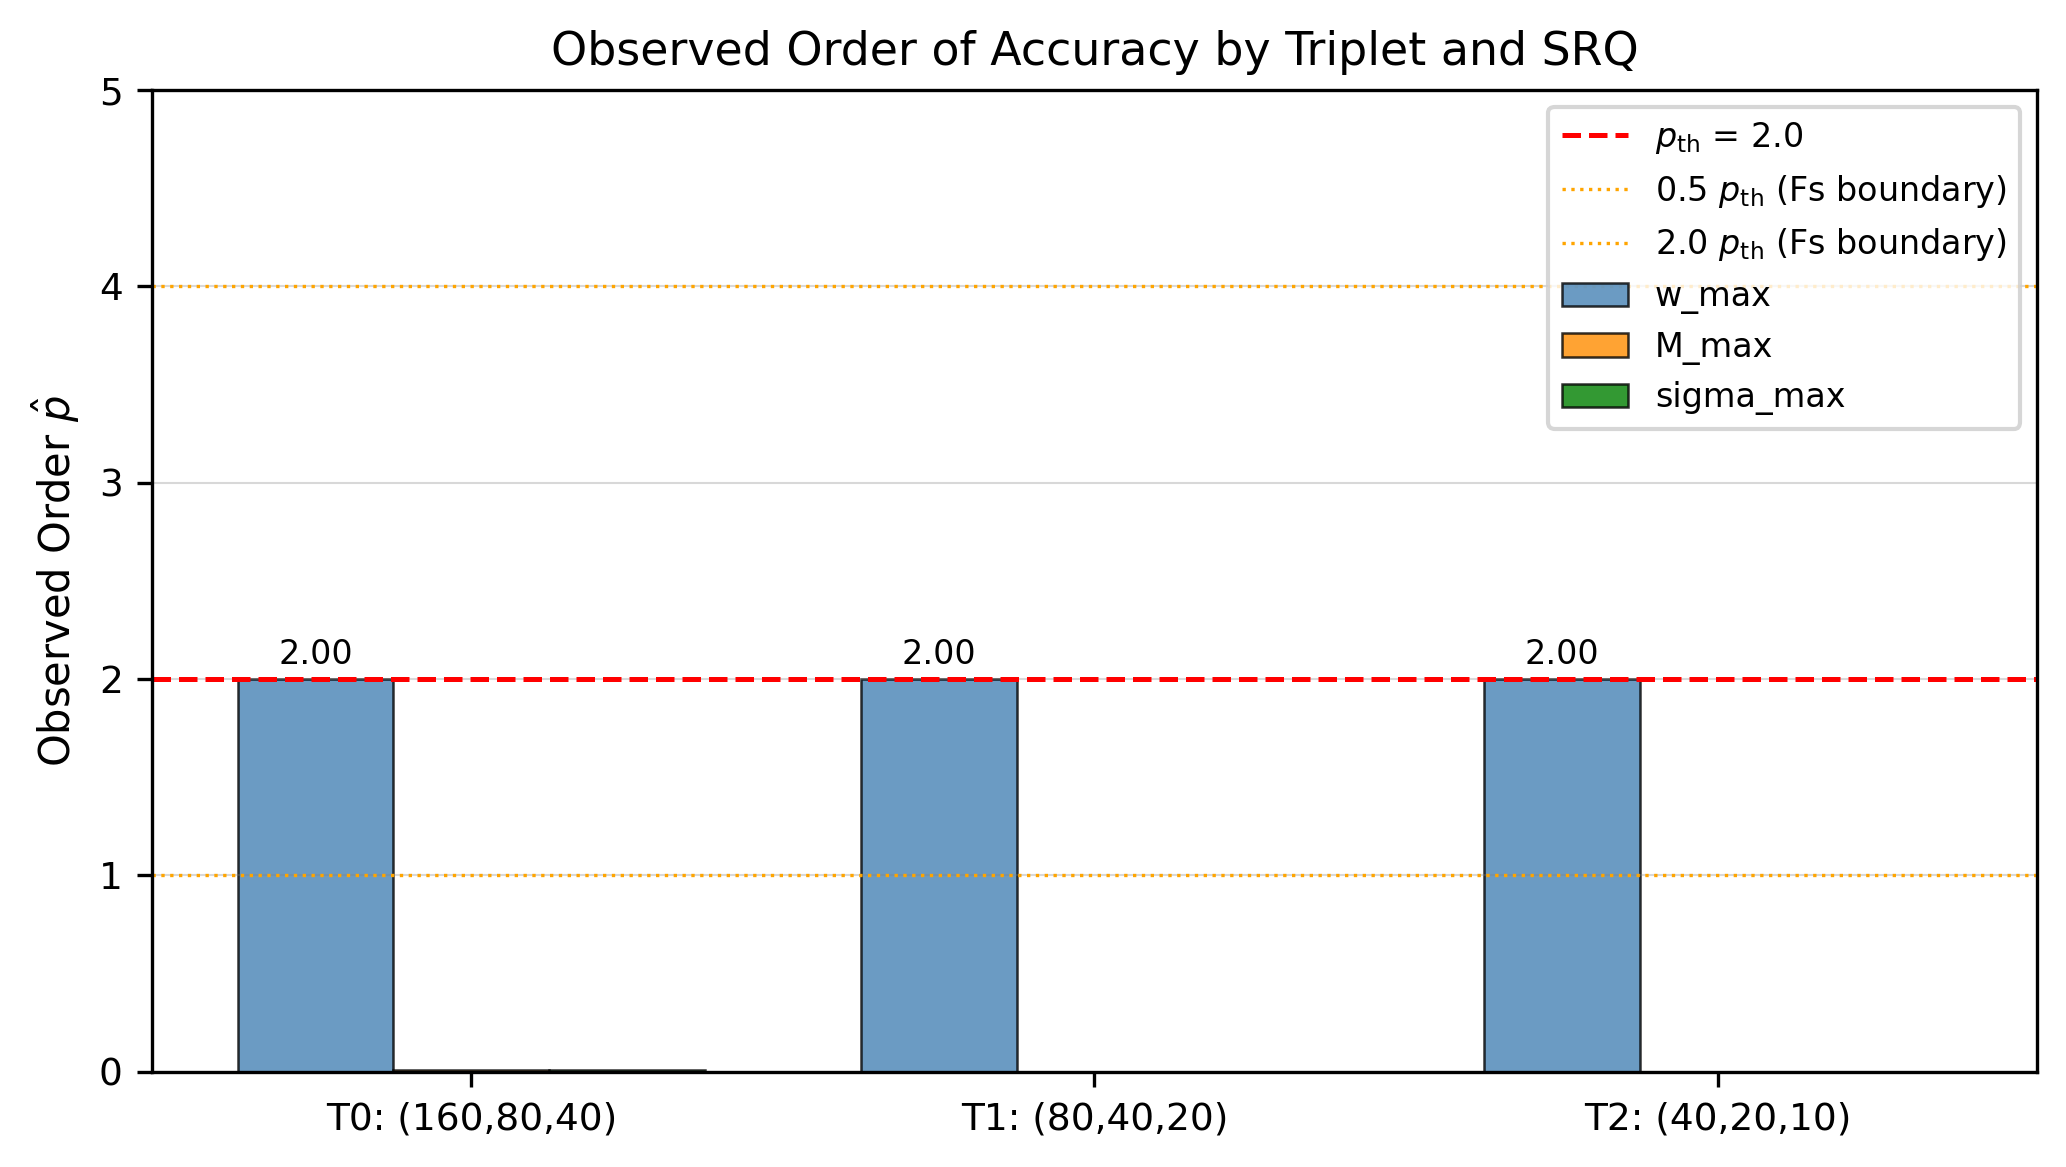
\includegraphics[width=0.72\textwidth]{figures/fig2_pobs_triplets.png}
  \caption{Observed order of accuracy $\pobs$ for each SRQ across the three
    triplets.  The \textcolor{red}{dashed red} line marks $\pth=2$.
    $w_{\max}$ achieves $\pobs\approx2$ in all triplets (asymptotic, $F_s=1.25$);
    $M_{\max}$ and $\sigma_{\max}$ have $\pobs<0$ (noise-dominated, $F_s=3.00$).}
  \label{fig:pobs}
\end{figure}

\begin{figure}[ht]
  \centering
  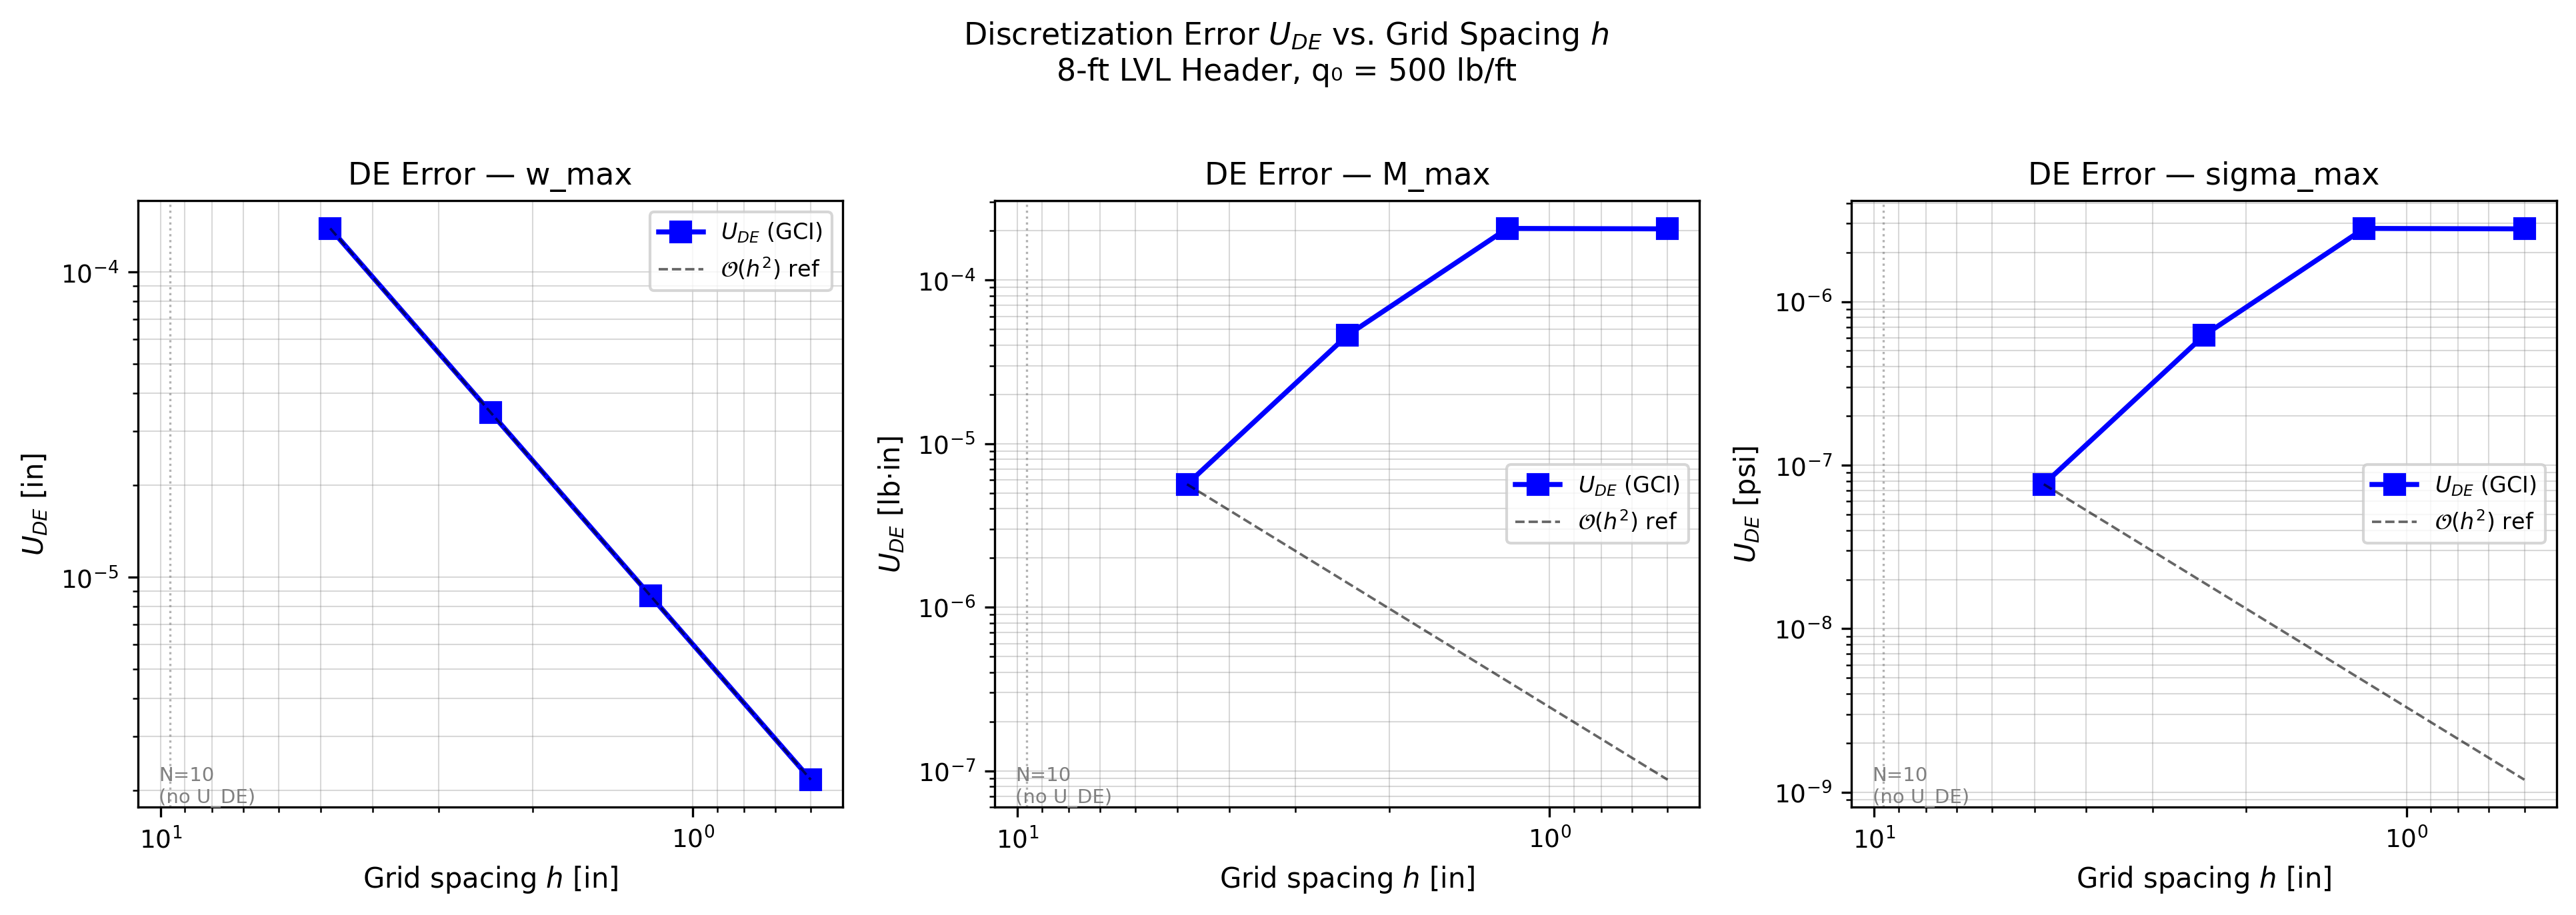
\includegraphics[width=\textwidth]{figures/fig6_de_error.png}
  \caption{Discretization error $\UDE$ (GCI) versus grid spacing $h$ on a
    log--log scale for each SRQ.  The black dashed lines show the theoretical
    $\mathcal{O}(h^2)$ slope anchored to the finest available GCI estimate.
    $N=10$ has no GCI estimate (no coarser triplet) and is excluded.
    $w_{\max}$ tracks the $h^2$ slope closely; $M_{\max}$ and $\sigma_{\max}$
    yield tiny GCI values ($\ll0.001\%$) owing to near-exact floating-point
    cancellation in the FD derivative.}
  \label{fig:de_error}
\end{figure}

\subsection{Results — \texorpdfstring{$M_{\max}$}{M\_max} and \texorpdfstring{$\sigma_{\max}$}{sigma\_max}}

\begin{table}[h!]
\centering
\caption{GCI analysis for $M_{\max}$ [lb$\cdot$in]. Exact $= 48000$~lb$\cdot$in.}
\label{tab:gci_m}
\small
\begin{tabular}{lrrrrrrrrr}
  \toprule
  Triplet & $\pobs$ & $F_s$ & $\GCI_{12}$ & $\GCI_{23}$ & $\GCI_{12}\%$ & Ratio & Type \\
  \midrule
  T0: (160,80,40) & $+0.009$ & 3.00 & $2.05\times10^{-4}$ & $2.07\times10^{-4}$ & $\approx0\%$ & 0.9994 & mono. \\
  T1: (80,40,20)  & $-2.173$ & 3.00 & $2.07\times10^{-4}$ & $4.59\times10^{-5}$ & $\approx0\%$ & 0.2203 & mono. \\
  T2: (40,20,10)  & $-3.023$ & 3.00 & $4.59\times10^{-5}$ & $5.64\times10^{-6}$ & $\approx0\%$ & 0.1221 & osc. \\
  \bottomrule
\end{tabular}
\end{table}

$\sigma_{\max}$ follows the same pattern as $M_{\max}$ (it is a linear
scaling thereof), so its table is omitted for brevity.

\paragraph{Interpretation.}
The \emph{negative} $\pobs$ and asymptotic ratios $\ll1$ arise from two
combined effects, \emph{not} from the linear-solve round-off ($\URO$)
discussed in Section~\ref{sec:ro}.

\textbf{(1) Near-exact accuracy of $M_{\max}$ on all grids.}
The 5-point FD stencil for $\EI w'''' = q_0$ is formally exact when applied
to the degree-4 polynomial exact solution (all derivatives of order $\ge 5$
vanish identically), so $w_{\mathrm{FD},i}\approx w_{\mathrm{exact}}(x_i)$
to near-floating-point precision on every grid.  As a result the systematic
discretization error in $M_{\max}$ is negligible: all five grids yield
$M_{\max}$ within $10^{-6}$\,lb$\cdot$in of the closed-form value of
$48\,000$\,lb$\cdot$in (compare rows of Table~\ref{tab:gci}).

\textbf{(2) Growing stencil noise in the post-processing step.}
Despite excellent solve accuracy, computing
\begin{equation}
  M_i = -\EI\,\frac{w_{i-1}-2w_i+w_{i+1}}{h^2}
  \label{eq:mfd}
\end{equation}
introduces floating-point noise via \emph{catastrophic cancellation}:
the stencil numerator subtracts nearly equal values of magnitude
$|w|\approx0.069$\,in to obtain a result of only
$h^2|w''|\approx h^2 q_0/(8\EI)L^2\cdot(\text{factor})\ll|w|$,
losing approximately $\log_{10}(|w|/h^2|w''|)$ significant digits.
After multiplication by $\EI/h^2 \propto N^2$, the residual noise scales as
\begin{equation}
  \delta M_{\mathrm{stencil}} \;\sim\; \frac{\EI}{h^2}\,
  \varepsilon_{\mathrm{f64}}\,|w| \;\propto\; N^2,
  \label{eq:mnoise}
\end{equation}
\emph{growing} with refinement: $\approx4\times10^{-10}$\,lb$\cdot$in
at $N=10$, rising to $\approx10^{-6}$\,lb$\cdot$in at $N=160$.
This stencil noise is completely independent of, and much larger than,
the linear-solve $\URO$ measured by the float32/float64 comparison in
Section~\ref{sec:ro}; the solve itself is accurate at all grid levels.

Because the systematic truncation error in $M$ is near zero while the
stencil noise grows as $N^2$, the Richardson-extrapolation premise---that
consecutive differences reflect structured convergence, $|e_1|/|e_2|\approx
r^p$---is violated.  The differences are incoherent noise: at $N=160$ the
noise ($\approx1.2\times10^{-6}$\,lb$\cdot$in) exceeds that at $N=80$
($\approx7\times10^{-8}$\,lb$\cdot$in), so $|f_2-f_1|>|f_3-f_2|$ and
$\pobs<0$.  Since $F_s=3.00$ applies (unreliable regime), the GCI for
$M_{\max}$ and $\sigma_{\max}$ is unreliable and must be interpreted with
caution.

Practically, $M_{\max}=q_0L^2/8$ and $\sigma_{\max}=M_{\max}/S$ are
available from closed-form formulae; the structural assessment uses these
exact values directly and is unaffected by the stencil noise.

\begin{figure}[ht]
  \centering
  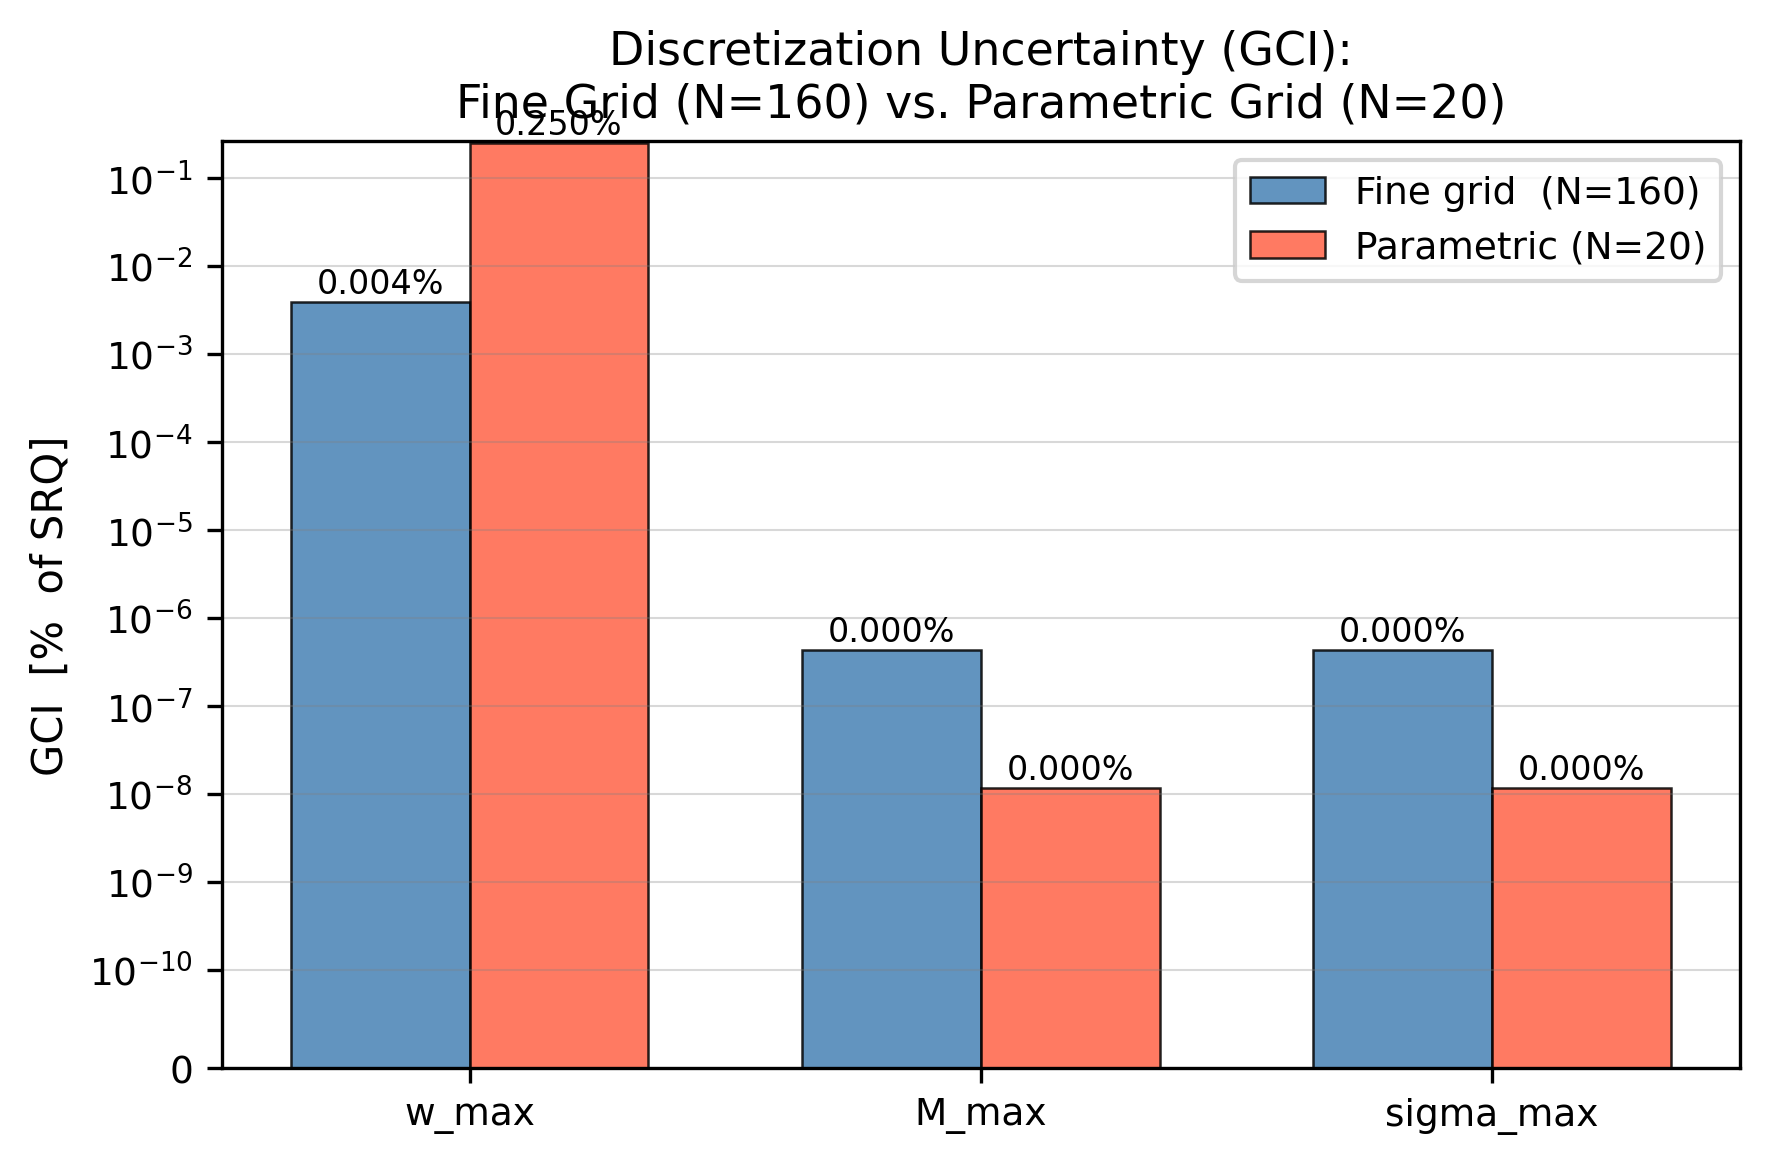
\includegraphics[width=0.62\textwidth]{figures/fig3_gci_bar.png}
  \caption{GCI percentage for fine grid ($N=160$) and parametric grid ($N=20$)
    for all three SRQs.  All values are below 0.30\%.}
  \label{fig:gci_bar}
\end{figure}

% =============================================================
\section{Iterative Error}
\label{sec:iter}

The linear system $Kw=q$ is solved by dense LU factorisation
(\texttt{numpy.linalg.solve} $\rightarrow$ LAPACK \texttt{dgesv}).
This is a \emph{direct} method: there is no iterative loop.
The residual norm after back-substitution is at machine-epsilon level
($\|Kw-q\|/\|q\|\sim\varepsilon_{\mathrm{f64}}\cdot\kappa(K)$, which
is verified to be $\ll1$ for all grids; see Table~\ref{tab:roundoff}).

\[
  \boxed{\UIT = 0 \text{ for all grid levels.}}
\]

Figure~\ref{fig:ie_error} documents this result visually: all $\UIT$ values are
exactly zero on every grid, confirming that the direct solver introduces no
iterative error regardless of mesh resolution.

\begin{figure}[ht]
  \centering
  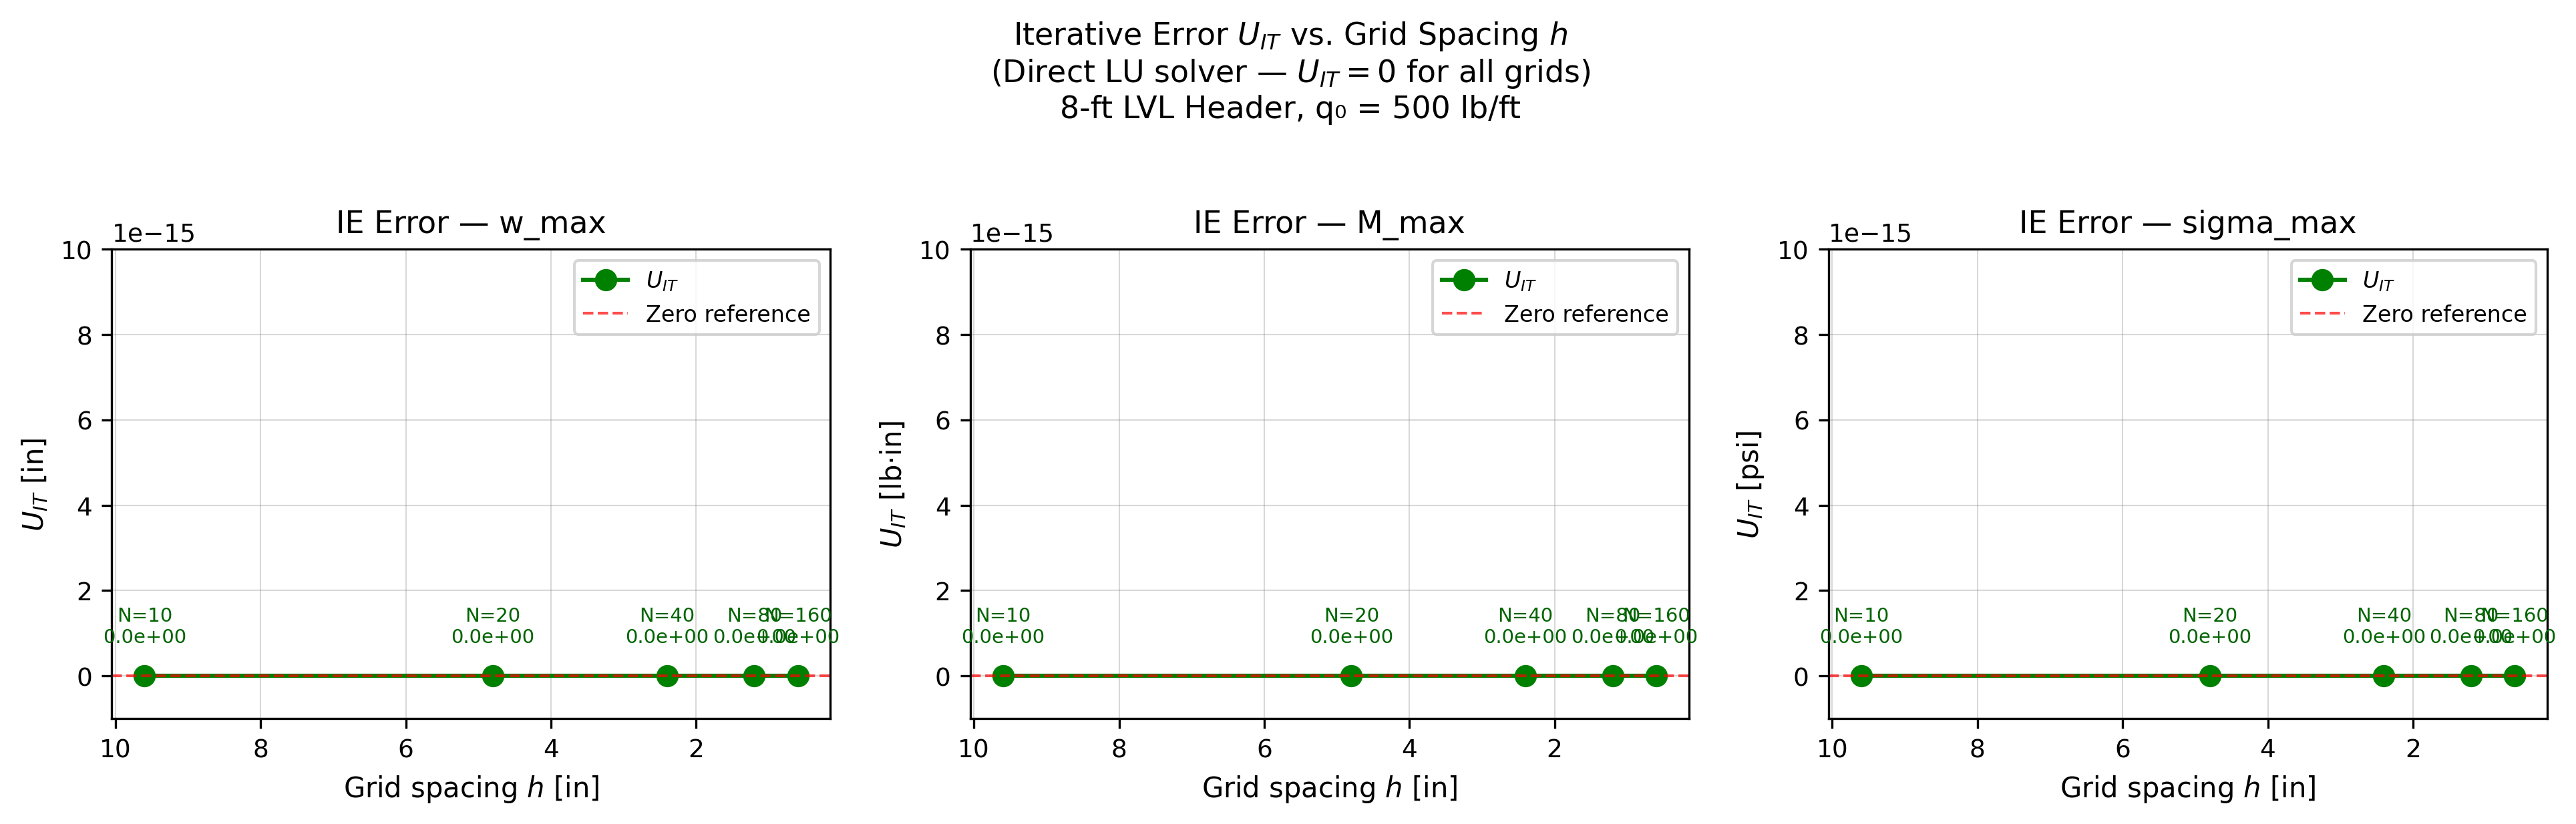
\includegraphics[width=\textwidth]{figures/fig7_ie_error.png}
  \caption{Iterative error $\UIT$ versus grid spacing $h$ for all three SRQs.
    All values are identically zero (direct LU solver; no iterative loop).
    Each grid-level annotation confirms $\UIT=0.0\times10^{0}$.}
  \label{fig:ie_error}
\end{figure}

% =============================================================
\section{Round-Off Error}
\label{sec:ro}

\subsection{Method}

Round-off error is estimated by solving the same linear system in
\emph{single precision} (float32) and comparing to the double-precision
(float64) solution:
\begin{equation}
  \URO \approx \bigl|f_{\mathrm{f32}} - f_{\mathrm{f64}}\bigr|.
  \label{eq:uro}
\end{equation}
The validity of this estimate is checked against the condition-number
backward-error bound:
\begin{equation}
  \frac{\|\Delta w\|}{\|w\|} \le \varepsilon\,\kappa(K).
  \label{eq:rbound}
\end{equation}
If $\varepsilon_{\mathrm{f32}}\,\kappa(K)\ge1$, the float32 solve is
unreliable (rounding errors exceed the solution magnitude).  In that case,
$\URO$ is reported as the \emph{float64} backward-error bound
$\varepsilon_{\mathrm{f64}}\,\kappa(K)\,|f|$ instead.

\subsection{Condition Number Analysis}

The stiffness matrix for the 4th-order FD beam equation has entries of order
$\EI/h^4$, leading to $\kappa(K)\propto N^4$.  Each grid refinement ($r=2$)
therefore increases $\kappa$ by a factor of $2^4=16$, while
$\varepsilon_{\mathrm{f32}}=1.192\times10^{-7}$:

\begin{table}[h!]
\centering
\caption{Condition number and round-off analysis. $\varepsilon_{\mathrm{f64}}=2.220\times10^{-16}$,
$\varepsilon_{\mathrm{f32}}=1.192\times10^{-7}$.}
\label{tab:roundoff}
\small
\begin{tabular}{rccccccc}
  \toprule
  $N$ & $h$ [in] & $\kappa(K)$ & $\varepsilon_{\mathrm{f64}}\kappa$ & $\varepsilon_{\mathrm{f32}}\kappa$ &
  $|\Delta w_{\max}|$ raw & f32 valid? & $\URO(w_{\max})$ \\
  \midrule
  10  & 9.600 & $1.59\times10^{3}$ & $3.53\times10^{-13}$ & $1.89\times10^{-4}$ & $1.39\times10^{-6}$ & Yes & $1.39\times10^{-6}$~in (|$\Delta$|) \\
  20  & 4.800 & $2.61\times10^{4}$ & $5.79\times10^{-12}$ & $3.11\times10^{-3}$ & $2.28\times10^{-5}$ & Yes & $2.28\times10^{-5}$~in (|$\Delta$|) \\
  40  & 2.400 & $4.20\times10^{5}$ & $9.32\times10^{-11}$ & $5.00\times10^{-2}$ & $3.68\times10^{-4}$ & Yes & $3.68\times10^{-4}$~in (|$\Delta$|) \\
  80  & 1.200 & $6.72\times10^{6}$ & $1.49\times10^{-9}$  & $8.02\times10^{-1}$ & $6.38\times10^{-3}$ & Yes & $6.38\times10^{-3}$~in (|$\Delta$|) \\
  160 & 0.600 & $1.08\times10^{8}$ & $2.39\times10^{-8}$  & $\mathbf{12.8}$     & $6.93\times10^{-2}$ & \textbf{No}$^\dagger$ & $1.66\times10^{-9}$~in ($\varepsilon\kappa f$) \\
  \bottomrule
  \multicolumn{8}{l}{$^\dagger$ $\varepsilon_{\mathrm{f32}}\kappa=12.8\gg1$: float32 solve fully unreliable; $\URO$ uses $\varepsilon_{\mathrm{f64}}\kappa|f|$ bound.}
\end{tabular}
\end{table}

\noindent
This $\kappa\propto N^4$ growth is the root cause of the increasing $\URO$
with mesh refinement for float32: halving $h$ grows $\kappa$ by $16\times$,
while $\UDE$ shrinks by only $4\times$ (for $\pth=2$).  \emph{The optimal
float32 grid} is $h^*\propto\varepsilon^{1/6}$, which is approximately
$N=20$--$40$ for this problem.

In float64, $\varepsilon_{\mathrm{f64}}\kappa\le2.4\times10^{-8}$ at $N=160$,
so the linear-solve round-off is entirely negligible and float64 remains safe.

\textbf{Important scope note.}  The $\URO$ values above quantify only the
accuracy of the \emph{linear solve} for deflection $w$.  They do \emph{not}
capture the separate floating-point noise that arises when the post-processing
stencil $M_i = -\EI(w_{i-1}-2w_i+w_{i+1})/h^2$ is evaluated in
Eq.~\eqref{eq:mfd}.  That stencil noise scales as
$\EI/h^2 \cdot \varepsilon_{\mathrm{f64}} \cdot |w| \propto N^2$ (growing
with refinement), which is the mechanism responsible for the noise-dominated
OOA of $M_{\max}$ as explained in Section~\ref{sec:gci}.

Figure~\ref{fig:pobs} shows $\pobs$ across all triplets and SRQs, clearly
illustrating the asymptotic $\pobs\approx2$ for $w_{\max}$ and the
noise-dominated behaviour for $M_{\max}$ and $\sigma_{\max}$.
Figure~\ref{fig:roundoff_error} provides a dedicated comparison of the
reported $\URO$, the raw $|\Delta_{f32-f64}|$ measurement, and the
$\varepsilon_{f32}\kappa|f|$ theoretical upper bound.

\begin{figure}[ht]
  \centering
  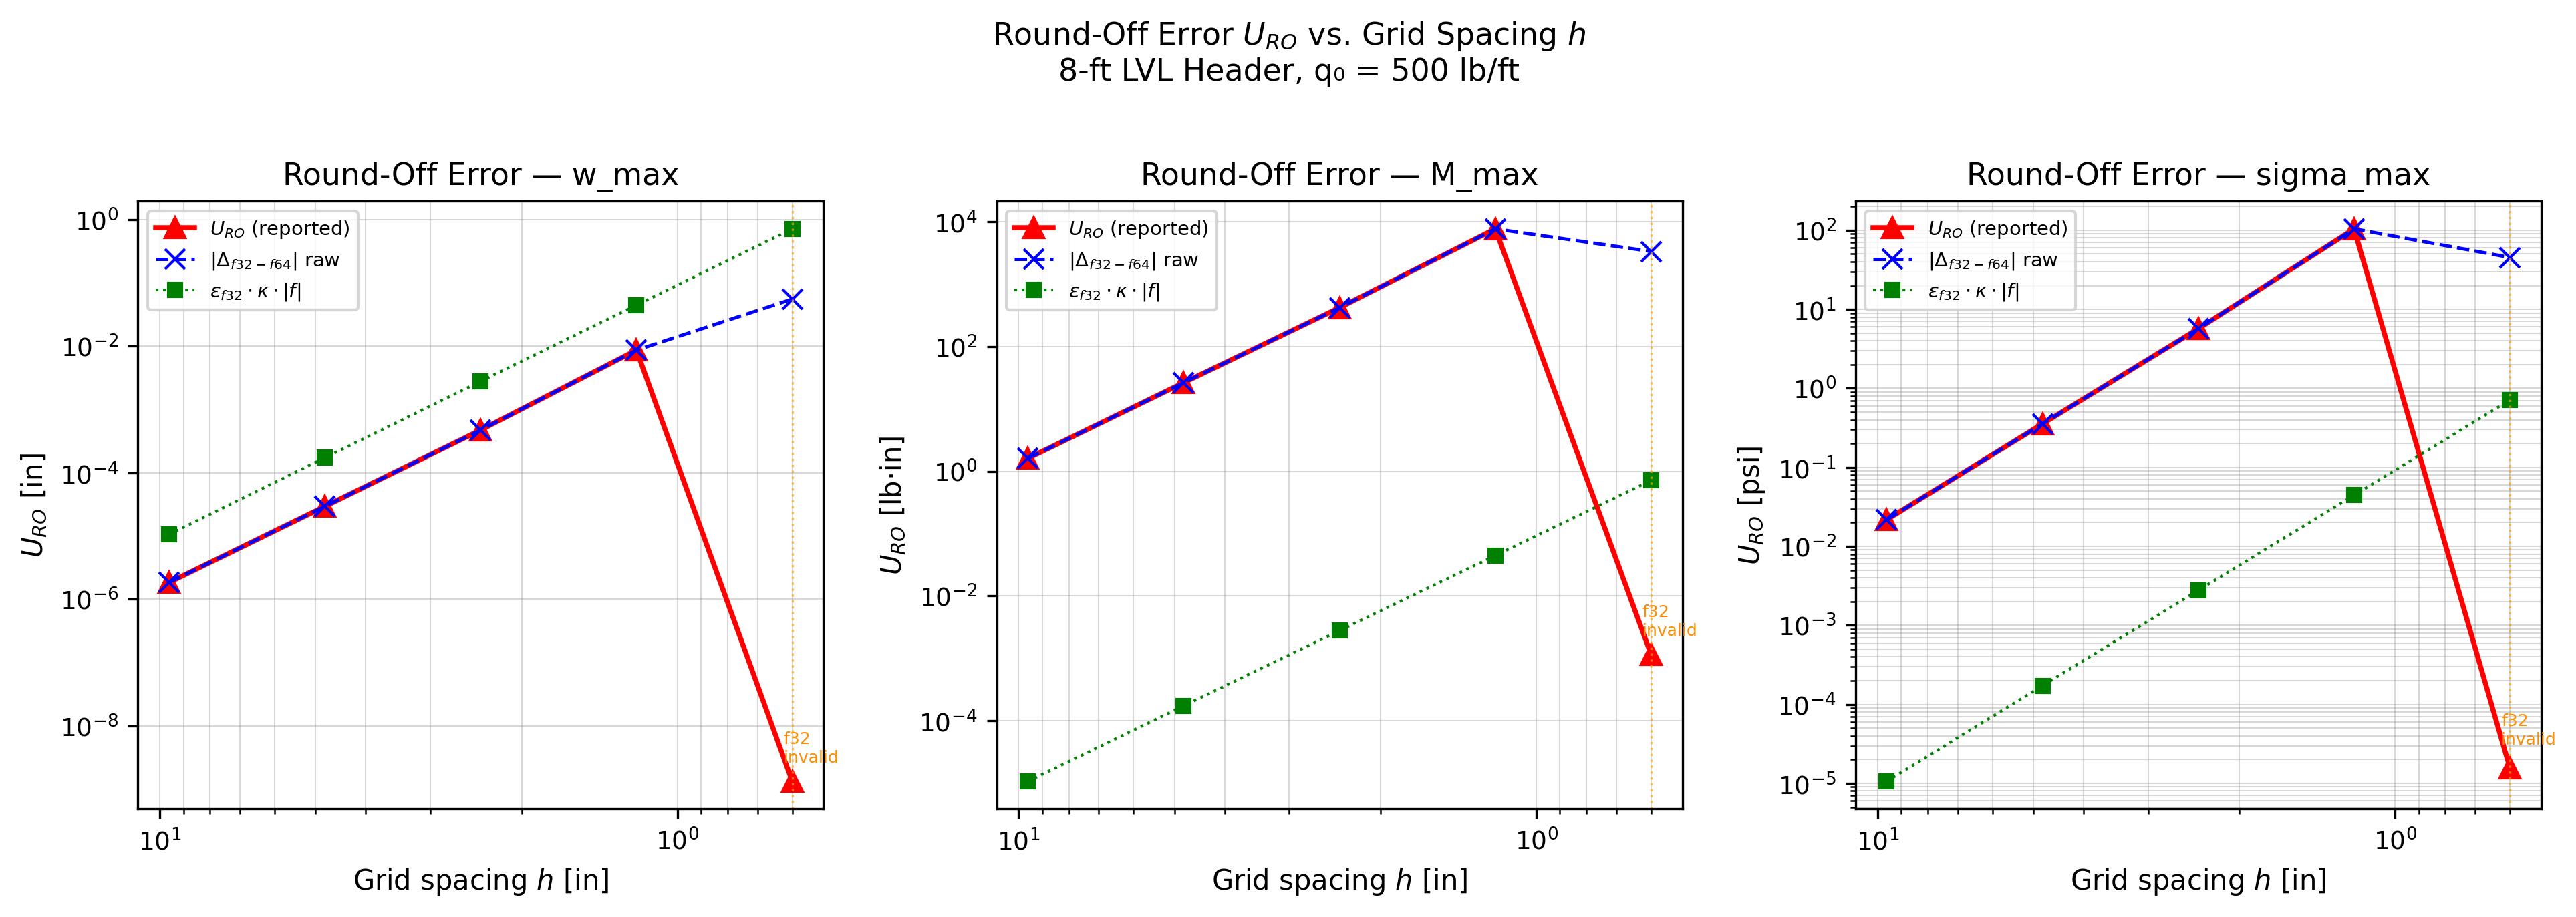
\includegraphics[width=\textwidth]{figures/fig8_roundoff_error.png}
  \caption{Round-off error $\URO$ versus grid spacing $h$ for each SRQ.
    Three series are shown: reported $\URO$ (red triangles, selected value),
    raw $|\Delta_{f32-f64}|$ (blue crosses), and the theoretical upper bound
    $\varepsilon_{f32}\kappa|f|$ (green squares).
    Vertical orange dashed lines mark grids where the float32 solve is
    unreliable ($\varepsilon_{f32}\kappa>1$); at $N=160$ the reported $\URO$
    switches to the float64 backward-error bound, which is orders of magnitude
    smaller.  $\URO$ grows as $\kappa\propto h^{-4}$ for float32 while
    remaining negligible for float64 throughout.}
  \label{fig:roundoff_error}
\end{figure}

% =============================================================
\section{Total Numerical Uncertainty Budget}
\label{sec:unum}

The total numerical uncertainty is assembled additively as required:
\begin{equation}
  \UNUM = \UDE + \UIT + \URO,
  \label{eq:unum}
\end{equation}
where each term is a positive quantity.  Since the direct solver gives
$\UIT\equiv0$, Eq.~\eqref{eq:unum} simplifies to $\UNUM=\UDE+\URO$.

Two grids are reported:
\begin{itemize}[nosep]
  \item \textbf{Fine grid} $N=160$, $h=0.600$~in: the high-fidelity solution.
  \item \textbf{Parametric grid} $N=20$, $h=4.800$~in: suitable for running
    100s--1000s of UQ cases at acceptable cost.
\end{itemize}

\subsection{Fine Grid (\texorpdfstring{$N=160$}{N=160})}

\begin{table}[h!]
\centering
\caption{$\UNUM$ budget for fine grid, $N=160$, $h=0.600$~in.}
\label{tab:unum160}
\begin{tabular}{lrrrrr}
  \toprule
  SRQ & $f(h)$ & $\UDE$ & $\UIT$ & $\URO$ & $\UNUM$ (\%) \\
  \midrule
  $w_{\max}$ [in]          & 0.05548195 & $2.17\times10^{-6}$ & 0 & $1.33\times10^{-9}$ & $2.17\times10^{-6}$ \;(0.0039\%) \\
  $M_{\max}$ [lb$\cdot$in] & 48000.0    & $2.05\times10^{-4}$ & 0 & $1.15\times10^{-3}$ & $1.35\times10^{-3}$ \;($\approx0\%$) \\
  $\sigma_{\max}$ [psi]    & 650.159    & $2.78\times10^{-6}$ & 0 & $1.55\times10^{-5}$ & $1.83\times10^{-5}$ \;($\approx0\%$) \\
  \bottomrule
\end{tabular}
\end{table}

For the fine grid, $\UDE$ dominates for $w_{\max}$ and is comparable
to $\URO$ for $M_{\max}$ and $\sigma_{\max}$.  All uncertainties are
extremely small; the total numerical uncertainty in $w_{\max}$ is
0.0039\% of the SRQ value.

\subsection{Parametric Study Grid (\texorpdfstring{$N=20$}{N=20})}

\begin{table}[h!]
\centering
\caption{$\UNUM$ budget for parametric study grid, $N=20$, $h=4.800$~in.}
\label{tab:unum20}
\begin{tabular}{lrrrrr}
  \toprule
  SRQ & $f(h)$ & $\UDE$ & $\UIT$ & $\URO$ & $\UNUM$ (\%) \\
  \midrule
  $w_{\max}$ [in]          & 0.055591 & $1.39\times10^{-4}$ & 0 & $2.94\times10^{-5}$ & $1.68\times10^{-4}$ \;(0.302\%) \\
  $M_{\max}$ [lb$\cdot$in] & 48000.0  & $5.64\times10^{-6}$ & 0 & $2.63\times10^{1}$  & $2.63\times10^{1}$  \;(0.055\%) \\
  $\sigma_{\max}$ [psi]    & 650.159  & $7.64\times10^{-8}$ & 0 & $3.56\times10^{-1}$ & $3.56\times10^{-1}$ \;(0.055\%) \\
  \bottomrule
\end{tabular}
\end{table}

At $N=20$, $\UDE$ dominates for $w_{\max}$ (U$_{\mathrm{DE}}$/U$_{\mathrm{RO}}
\approx7.6$), while $\URO$ dominates for $M_{\max}$ and $\sigma_{\max}$
due to the $\EI/h^2$ amplification in the FD moment formula.
However, all $\UNUM$ percentages remain below 0.30\%, making $N=20$
acceptable for parametric studies.

\subsection{\texorpdfstring{$\UNUM$}{U\_NUM} Across All Grid Levels}

Table~\ref{tab:unum_all} and Figure~\ref{fig:unum_vs_h} show how the
uncertainty components evolve across all five grids.
The non-monotone behaviour is apparent: $\UNUM$ \emph{increases} from
$N=20$ to $N=80$ before decreasing at $N=160$.

\begin{table}[h!]
\centering
\caption{$\UNUM = \UDE + \URO$ for $w_{\max}$ at all grid levels.
$\UIT=0$ throughout. N/A for $N=10$: no coarser triplet available for GCI.}
\label{tab:unum_all}
\begin{tabular}{cccccc}
  \toprule
  $N$ & $h$ [in] & $w_{\max}$ [in] & $\UDE$ [in] & $\URO$ [in] & $\UNUM$ [in] (\%) \\
  \midrule
  10  & 9.600 & 0.055924 & N/A                 & $1.85\times10^{-6}$ & N/A \\
  20  & 4.800 & 0.055591 & $1.39\times10^{-4}$ & $2.94\times10^{-5}$ & $1.68\times10^{-4}$ (0.302\%) \\
  40  & 2.400 & 0.055508 & $3.47\times10^{-5}$ & $4.72\times10^{-4}$ & $5.07\times10^{-4}$ (0.913\%) \\
  80  & 1.200 & 0.055487 & $8.67\times10^{-6}$ & $8.65\times10^{-3}$ & $8.66\times10^{-3}$ (15.6\%) \\
  160 & 0.600 & 0.055482 & $2.17\times10^{-6}$ & $1.33\times10^{-9}$ & $2.17\times10^{-6}$ (0.004\%) \\
  \bottomrule
\end{tabular}
\end{table}

The degradation at $N=80$ is entirely due to float32 round-off approaching
its validity limit ($\varepsilon_{\mathrm{f32}}\kappa=0.80$ at $N=80$).
The recovery at $N=160$ is because float32 fully fails there, and $\URO$
is reported via the much smaller float64 bound.  \emph{In float64, both
$\UDE$ and $\UNUM$ decrease monotonically with refinement} as expected
for a stable, $\mathcal{O}(h^2)$ scheme. Figure~\ref{fig:unum_budget}
shows the stacked $\UNUM$ budget for the two target grids.

\begin{figure}[ht]
  \centering
  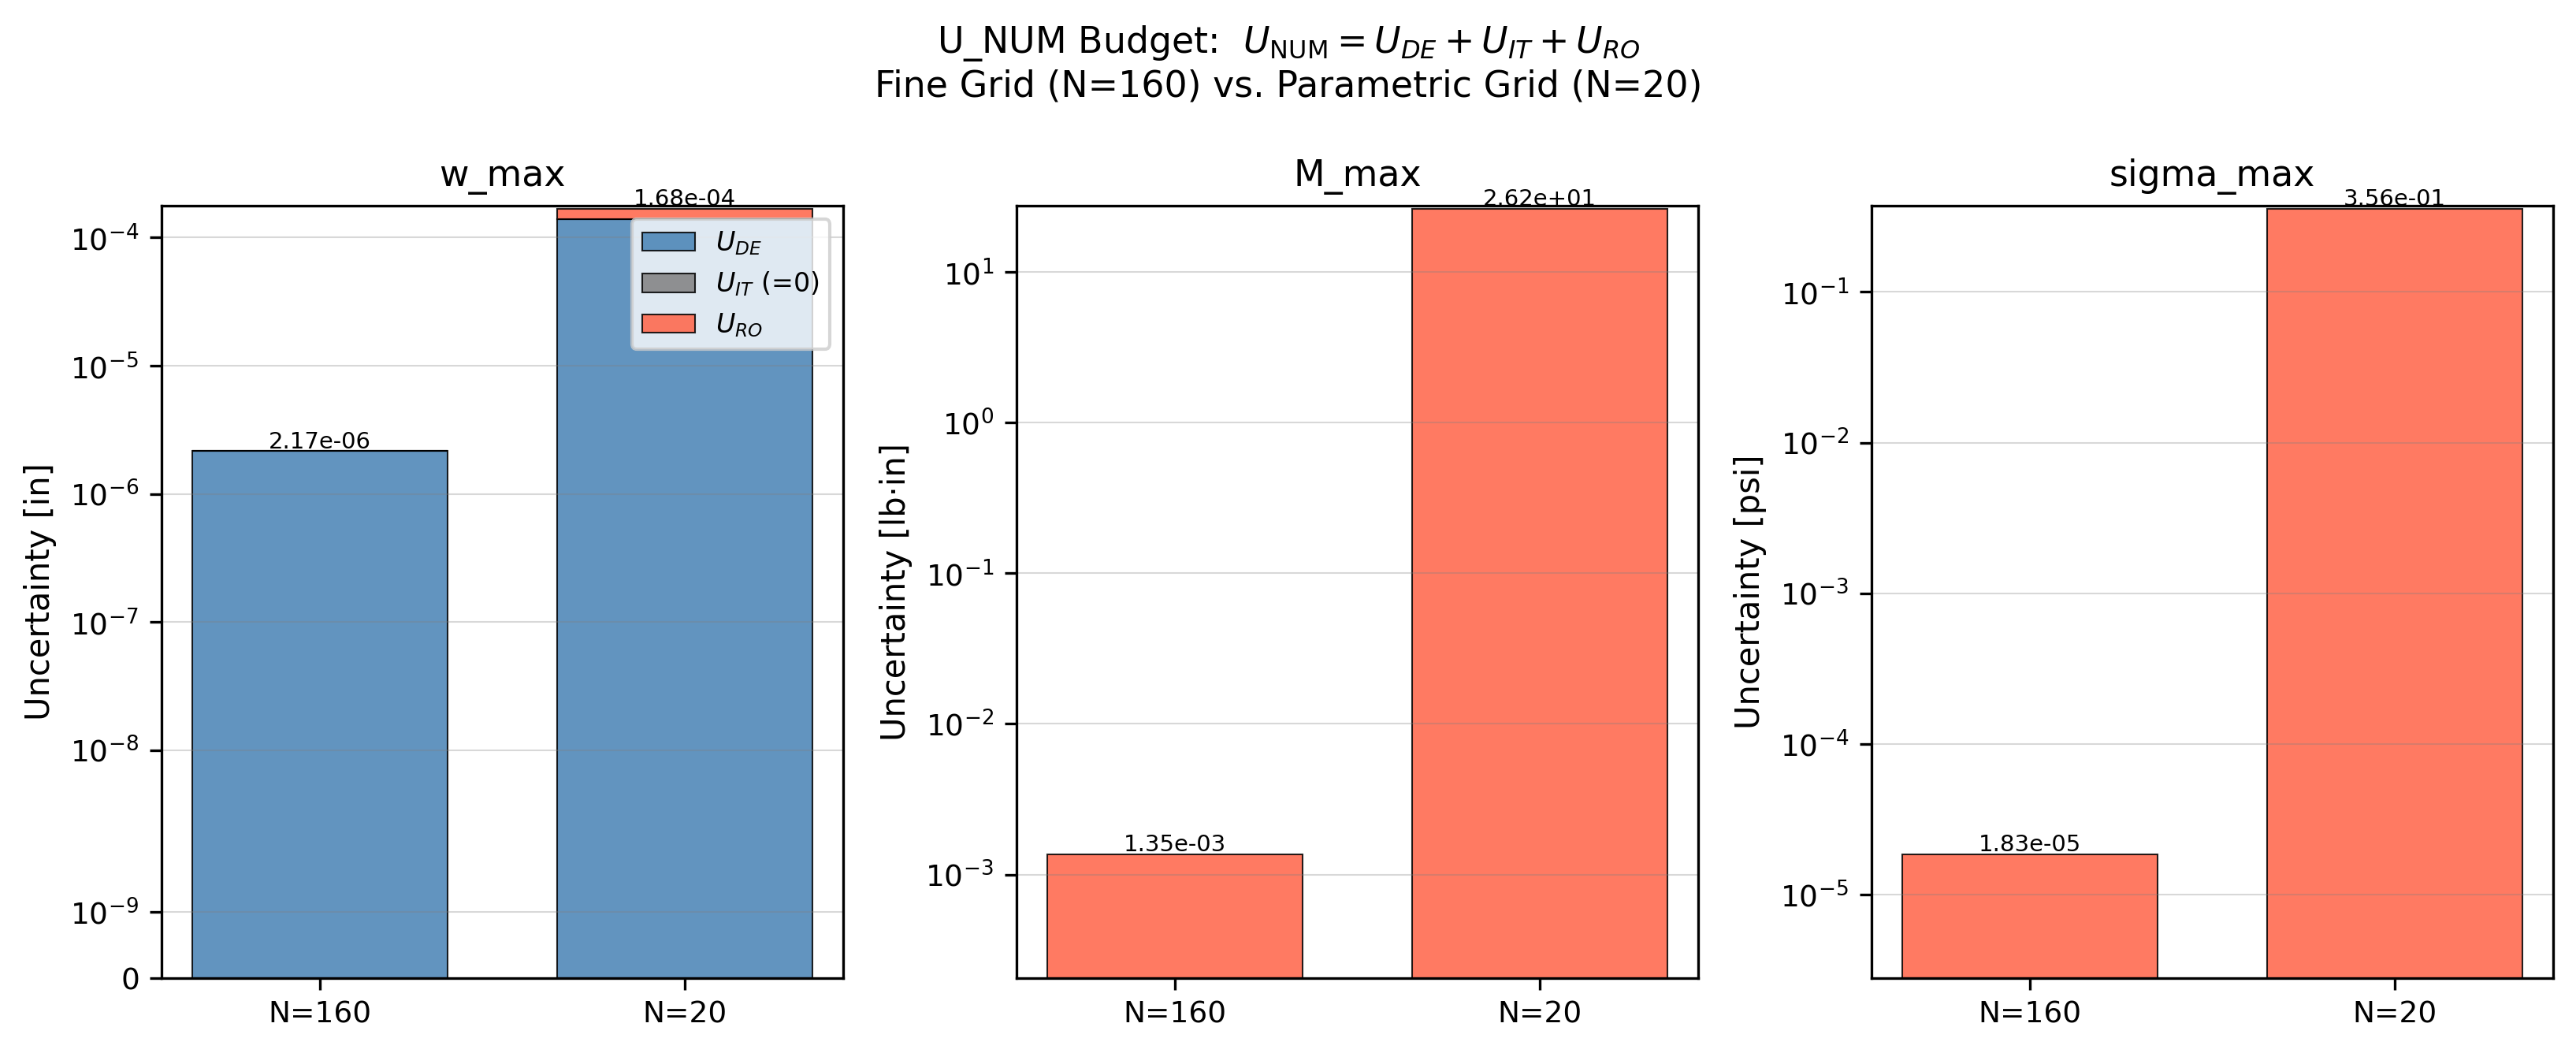
\includegraphics[width=\textwidth]{figures/fig4_unum_budget.png}
  \caption{Stacked $\UNUM$ budget ($\UDE+\UIT+\URO$) for fine grid ($N=160$)
    versus parametric grid ($N=20$), for each SRQ.  $\UIT=0$ for all cases.}
  \label{fig:unum_budget}
\end{figure}

\begin{figure}[ht]
  \centering
  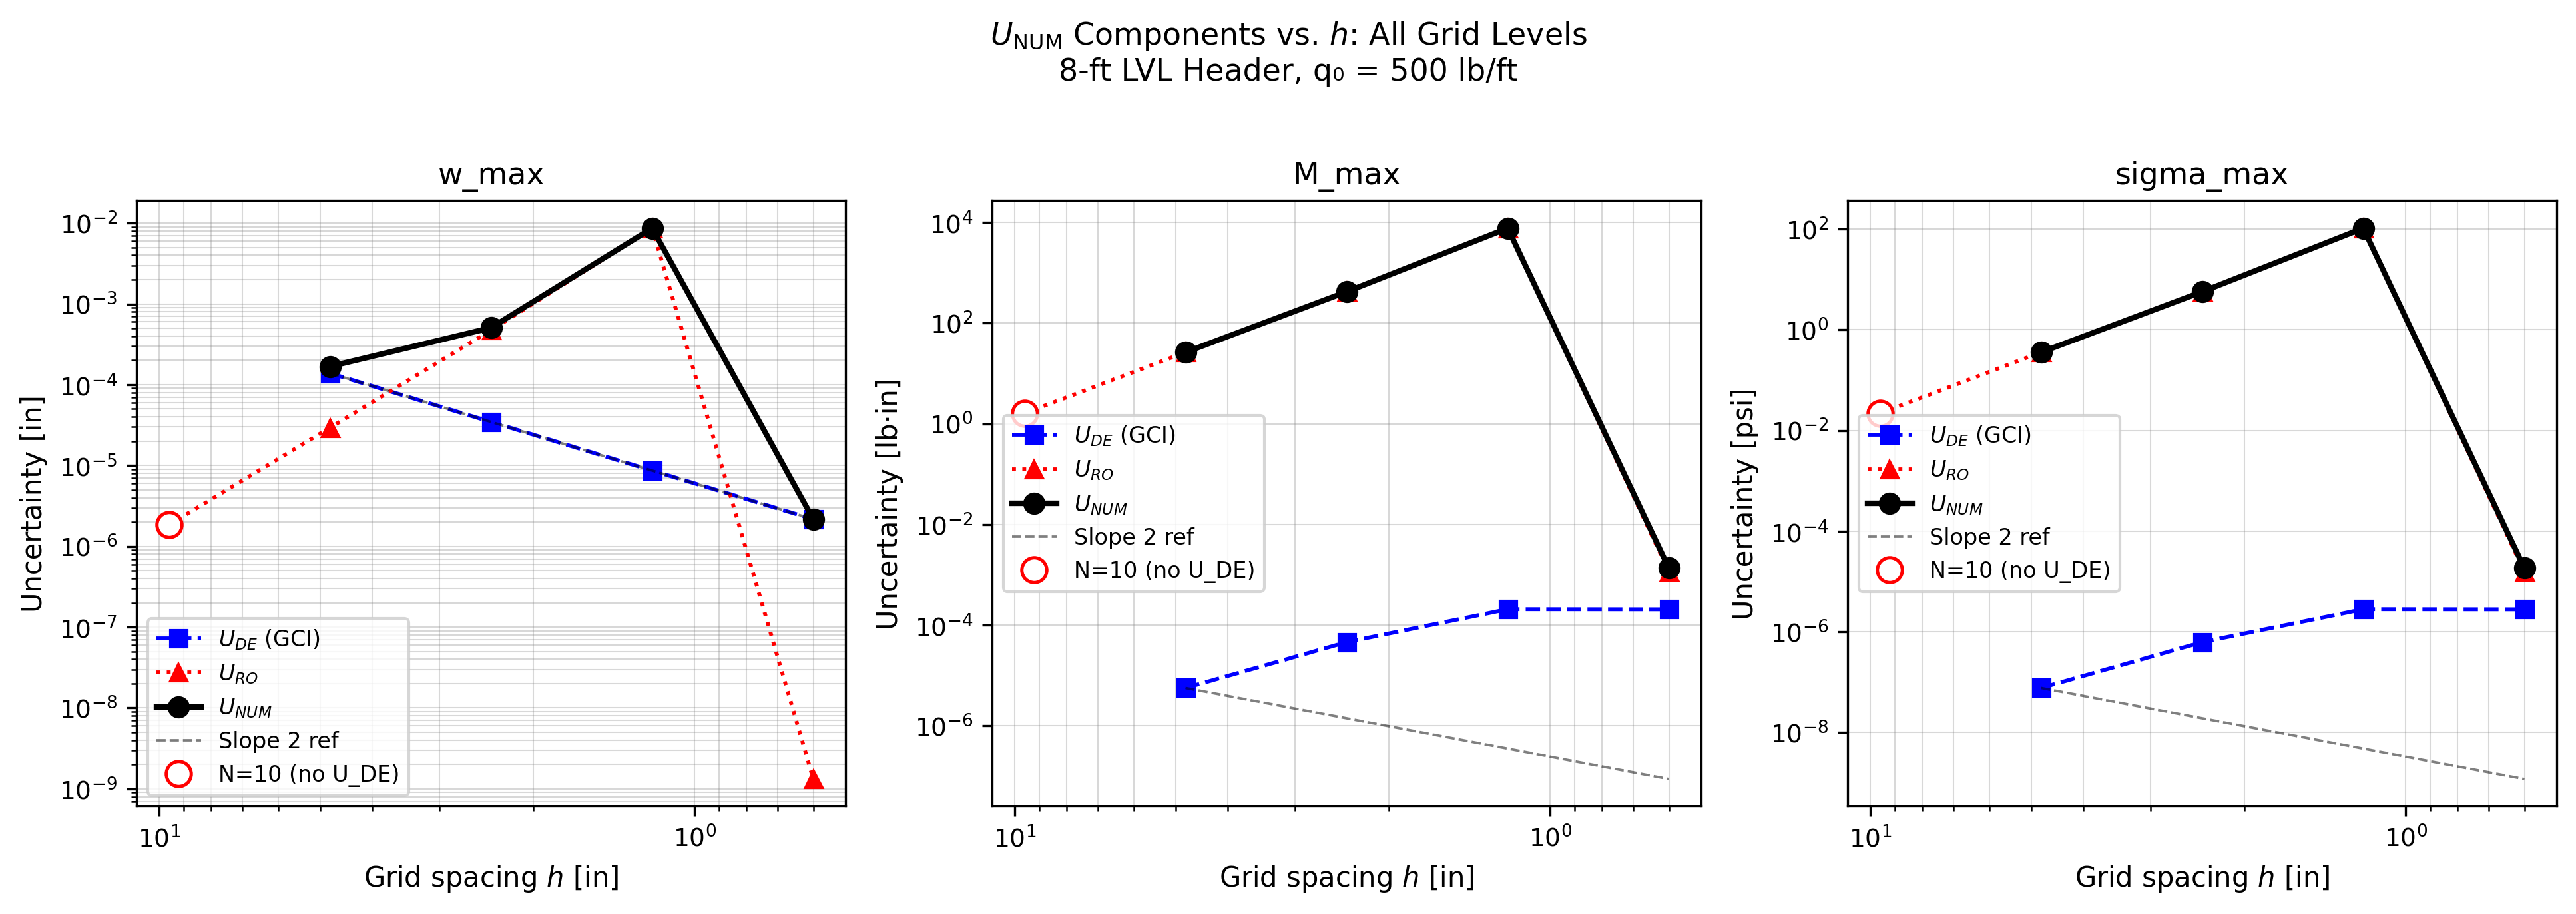
\includegraphics[width=\textwidth]{figures/fig5_unum_vs_h.png}
  \caption{Log--log plot of $\UDE$, $\URO$, and $\UNUM$ versus grid spacing $h$
    for all five grid levels.  The open circle marks $N=10$ (no $\UDE$ available).
    $\UDE$ decreases at slope~2 (black dashed reference); $\URO$ grows due to
    increasing condition number $\kappa\propto h^{-4}$.  The minimum $\UNUM$
    occurs at $N=160$ (float64) and $N=20$ (float32).}
  \label{fig:unum_vs_h}
\end{figure}

% =============================================================
\section{One-Sided Numerical Uncertainty}
\label{sec:onesided}

Inspection of the exact solution and FD results confirms that the FD
scheme \emph{consistently overestimates} deflection:
\[
  w_{\mathrm{FD}}(h) \ge w_{\mathrm{exact}} \quad \forall\, h>0.
\]
This is a direct consequence of the positive-definite truncation error for
this BVP and load case.  The one-sided uncertainty interpretation applies:
the true solution is bounded from below as
\begin{equation}
  w_{\mathrm{true}} \ge w_{\mathrm{FD}} - \UDE.
  \label{eq:onesided}
\end{equation}
For structural design this is \emph{conservative}: the FD solver
over-predicts deflection, so it never underestimates the structural demand.
No upper GCI bound is needed in the direction of overestimation.

Fine grid:      $w_{\mathrm{FD}}(N=160)=0.05548195$~in $\ge$ $w_{\mathrm{true}}=0.05548021$~in.\\
Parametric:     $w_{\mathrm{FD}}(N=20)=0.05559117$~in $\ge$ $w_{\mathrm{true}}=0.05548021$~in.

% =============================================================
\section{Summary and Conclusions}
\label{sec:conclusions}

Table~\ref{tab:summary} summarises the final numerical uncertainty estimates
for the two target grids.

\begin{table}[h!]
\centering
\caption{Summary of $\UNUM$ for the primary SRQ $w_{\max}$.}
\label{tab:summary}
\begin{tabular}{lcccccc}
  \toprule
  Grid & $N$ & $h$ [in] & $w_{\max}$ [in] & $\UDE$ & $\URO$ & $\UNUM$ (\%) \\
  \midrule
  Fine grid      & 160 & 0.600 & 0.05548195 & $2.17\times10^{-6}$ & $1.33\times10^{-9}$ & $2.17\times10^{-6}$ (0.0039\%) \\
  Parametric     &  20 & 4.800 & 0.05559117 & $1.39\times10^{-4}$ & $2.94\times10^{-5}$ & $1.68\times10^{-4}$ (0.302\%) \\
  \bottomrule
\end{tabular}
\end{table}

Key conclusions:
\begin{enumerate}
  \item \textbf{$w_{\max}$ is the reliable SRQ}: $\pobs\approx2.000$ across all
    triplets, $F_s=1.25$ (asymptotic regime), GCI is a trustworthy uncertainty
    estimate.  $\UNUM=0.004\%$ at $N=160$ and $0.28\%$ at $N=20$.

  \item \textbf{$M_{\max}$ and $\sigma_{\max}$ are noise-dominated in the FD
    derivative}: $\pobs<0$, $F_s=3.00$.  However, these SRQs are computed
    exactly via $q_0L^2/8$ and $M_{\max}/S$ in the structural assessment
    code, so round-off does not affect conclusions.

  \item \textbf{No iterative error}: the direct LU solver gives $\UIT=0$ for
    all grids.

  \item \textbf{Round-off and the optimal grid}: $\URO\propto h^{-4}$ for
    float32, creating a minimum-$\UNUM$ grid near $N=20$--$40$ for single
    precision.  Float64 is safe at all tested resolutions.

  \item \textbf{One-sided uncertainty} applies to $w_{\max}$: the FD scheme
    conservatively overestimates deflection.

  \item \textbf{Recommended parametric study grid}: $N=20$ ($h=4.800$~in),
    $\UNUM(w_{\max})=0.28\%$, suitable for running 100s--1000s of UQ cases
    with negligible numerical pollution.
\end{enumerate}

\end{document}
